\section{Heurystyka single swap}

W tym podrozdziale opiszemy heurystykę single swap \cite{Arya2004LocalSH}, która jest przykładem techniki \textit{local search}.
Metoda local search jest heurystyką, która zaczyna od dowolnego rozwiązania $S$ problemu optymalizującego.
Następnie sprawdza czy niewielka zmiana rozwiązania $S$ poprawia wartość funkcji celu problemu.
Jeżeli tak, to wykonuje tę zmianę.
Heurystyka kończy swoje działanie w momencie kiedy zmiana w rozwiązaniu nie poprawia funkcji celu.
W efekcie otrzymujemy lokalnie optymalne rozwiązanie dla danego na wejściu problemu optymalizującego.
Algorytm jest 25-aproksymacją problemu $k$-means, która zakłada, że na wejściu dostajemy zbiór kandydatów na centra $C$ oraz zbiór $n$ punktów $P \subset \mathbb{R}^d$.
Autorzy \cite{Arya2004LocalSH} w celu wyznaczenia $C$ wykorzystują algorytm z pracy \cite{Matousek99onapproximate}, którą zastąpimy pracą \cite{10.1145/1007352.1007400} z uwagi na lepsze gwarancje teoretyczne.
Korzystając z algorytmu opisanego w podrozdziale 4.2.3 wyznaczamy zbiór $C$, który będzie obliczonym $(\epsilon, k)$-coresetem.
\\~\\
Heurystyka \textit{single swap} działa poprzez wybranie początkowego zestawu $k$ centrów $S$ ze zbioru kandydatów na centra $C$, a następnie wielokrotnej
próbie ulepszenia rozwiązania poprzez usunięcie jednego centrum $s \in S$ i zastąpienie go innym centerm $s^{'} \in C - S$.
Początkowy stan $S$ może zostać zainicjalizowany losowo albo może być obliczony za pomocą omówionego w podrozdziale 4.1 algorytmu Gonzaleza.
Niech $S^{'} = S - \{s\} \cup \{s^{'}\}$ będzie nowym zbiorem centrów, gdzie taką operację na zbiorze $S$ nazwyamy \textit{wymianą} a punkty $s$, $s^{'}$ \textit{swap parą}.
Jeżeli $\phi_{P}(S^{'}) \leq \phi_{P}(S)$ to zastępujemy zbiór $S$ zbiorem $S^{'}$, w przeciwnym przypadku $S$ pozostaje bez zmian.
W praktyce taki proces powtarzamy do momentu, kiedy $|\phi_{P}(S^{'}) - \phi_{P}(S) | < \epsilon$.
Formalnie można udowodnić, że dla każdego $\epsilon > 0$, po wielomianiwej liczbie wymian punktów $s$, $s^{'}$ algorytm zakończy swoje działanie.
Autorzy nie dowodzą tego wprost ale powołują się na pracę \cite{10.1145/380752.380755}.
\\~\\
Dla uproszczenia zakładamy, że algorytm kończy się kiedy pojedyńcza wymiana elementów $s$, $s^{'}$ nie poprawia wyniku.
Taki zbiór centrów nazwiemy \textit{1-stable}.
\\~\\
Wprowadźmy notację:
\begin{equation}
    \Delta(u, v) = d(u, v)^{2} = \sum_{i=0}^{d} (u_{i} - v_{i})^2 = (u - v)\cdot(u - v)
\end{equation}
gdzie punkty interpretujemy jako wektory oraz operacja $(\cdot)$ jest iloczynem skalarnym.
\begin{equation}
    \Delta(S, v) = \sum_{u \in S} d(u, v)^{2}
\end{equation}
\begin{equation}
    \phi_{P}(S) = \Delta(S) = \sum_{q \in P} \Delta(q,s_{q}) = \sum_{q \in P} d(q, s_{q})^{2}
\end{equation}
gdzie $s_{q}$ to najbliższy punkt dla $q$ w $S$ oraz $P \subset \mathbb{R}^{d}$. 

\begin{definition}
    Zbiór $S$ nazywamy \emph{1-stable}, jeżeli:
    \begin{equation}
        \Delta(S - \{s\} \cup \{c\}) \leq \Delta(S)
    \end{equation}
    dla dowolnych $s \in S$ oraz $c \in C_{opt}$.
\end{definition}

\begin{definition}
    Niech $N_{S}(s)$ oznacza sąsiedzctwo punktu $s$, czyli zbiór punktów z $P$, dla których punkt $s$ jest najbliżej spośród punktów z $S$.
\end{definition}

\noindent
Autorzy pracy \cite{Arya2004LocalSH} w analizie powołują się na kryterium dla lokalnej minimalności rozwiązania problemu $k$-means \cite{doi:10.1137/S0036144599352836}.
Mówi ono, że dla dowolnego lokalnie minimalnego rozwiązania $C_{min}$ problemu $k$-means, każde centrum $c_{i} \in C_{min}$ jest centroidem jego sąsiedztwa.
Rozwiązanie $C_{min}$ nazywamy \textit{centroidalnym}.
Zatem, ponieważ punkty interpretujemy jak wektory oraz z powyższego kryterium:
\begin{equation}
    s = \frac{1}{|N_{S}(s)|}\sum_{u \in N_{S}(s)} u
\end{equation}
\\~\\
W ramach tego podrozdziału udowodnimy następujące twierdzenie.

\begin{thm}{\cite{Arya2004LocalSH}}
    Niech $S$ będzie zbiorem $k$ punktów spełniającym definicję 1-stable oraz niech $C_{opt}$ będzie optymalnym zbiorem dla problemu $k$-means.
    Wtedy zachodzi następującą nierówność:
    \begin{equation}
        \Delta(S) \leq 25 \Delta(C_{opt})
    \end{equation} 
\end{thm}

\begin{lemma}{\cite{Arya2004LocalSH}}
    Dla danego skończonego podzbioru $S$ punktów z $\mathbb{R}^d$, niech $c$ będzie centroidem dla $S$. Wtedy dla dowolnego $c^{'} \in \mathbb{R}^d$, $\Delta(S, c^{'}) = \Delta(S, c) + |S|\Delta(c, c^{'})$.
\end{lemma}
\begin{proof}
    Z definicji $\Delta(S, c^{'})$ otrzymujemy:
    \begin{equation}
        \Delta(S, c^{'}) = \sum_{u \in S} \Delta(u, c^{'}) =  \sum_{u \in S} (u - c^{'}) (u - c^{'})
    \end{equation}
    \begin{equation}
         = \sum_{u \in S} ((u - c) + (c - c^{'})) ((u - c) + (c - c^{'}))
    \end{equation}
    \begin{equation}
        = \sum_{u \in S} ((u - c)(u - c)) + 2((u - c)(c - c^{'})) + ((c - c^{'})(c - c^{'}))
    \end{equation}
    \begin{equation}
        = \Delta(S, c) + 2\Big( (c - c^{'}) \sum_{u \in S} (u - c) \Big) + |S|((c - c^{'})(c - c^{'}))
    \end{equation}
    \begin{equation}
        = \Delta(S, c) + |S|\Delta(c,c^{'})
    \end{equation}
    Ostanie przejście korzysta z faktu, że jeżeli $c$ jest centroidem $S$ to z definicji zachodzi $\sum_{u \in S} (u - c) = 0$.
\end{proof}

%\epsilon
\noindent
Na potrzebę dowodu załóżmy, że znamy zbiór $C_{opt}$.
Dla każdego optymalnego $c \in C_{opt}$ wyznaczamy $s_{c}$, który jest najbliższym punktem w $S$ dla punktu $c$.
Punkt $s_{c}$ nazywamy heurystycznym centrum dla punktu $c$.
W takim kontekście powiemy, że $c$ jest \textit{schwytane} przez $s_{c}$.
Tutaj warto zaznaczyć, że każde optymalne centrum jest schwytane przez jedno heurystyczne centrum, ale każde heurystyczne centrum może chwytać kilka optymalnych centrów.
Heurystyczne centrum nazwiemy \textit{samotnym} jeżeli nie chwyta żadne optymalne centrum.

\begin{proof}
    Dowód twierdzenia 4.2 zaczniemy od zdefniowania podziału $S$ oraz $C_{opt}$ na zbiory $S_{1}, \dots, S_{r}$ oraz $O_{1}, \dots, O_{r}$ dla pewnego $r$, gdzie $|S_{i}| = |O_{i}|$ dla $i = 1, \dots, r$.
    \\~\\
    Dla każdego heurystycznego centrum $s_{i}$, które schywało jakąś liczbę $m \geq 1$ optymalnych centrów, tworzymy zbior $S_{i}$, który będzie zawierał $s_{i}$ oraz dowolne $m-1$ osamotnionych heurystycznych centrów.
    Analogicznie, zbior $O_{i}$ będzie zawierał wszystkie optymalne centra schwytane przez $s_{i}$.
    Rysunek 4.2 obrazuje tak zdefiniowany podział.
    \\~\\
    \noindent
    Wygenerujemy teraz \textit{swap par} dla utworzonego podziału.
    Dla każdego podzbioru podziału takiego, że $|S_{i}| = |O_{i}| = 1$ , tworzymy z ich elementów parę.
    Dla każdego podzbioru podziału, który zawiera więcej schwytanych centrów, czyli $|S_{i}|, |O_{i}| \geq 1$, tworzymy pary między osamotnionymi heurystycznymi centrami z $S_{i}$ a optymalnymi centrami z $O_{i}$.
    Każde optymalne centrum jest związane z jednym heurystycznym oraz każde osamotnione centrum jest przyporządkowane co najwyżej dwóm optymalnym centrom.
    Centra łaczymy dowolnie. 
    Rysunek 4.2 przedstawia przykładowe swap pary.
    \begin{figure}[H]
        \centering
        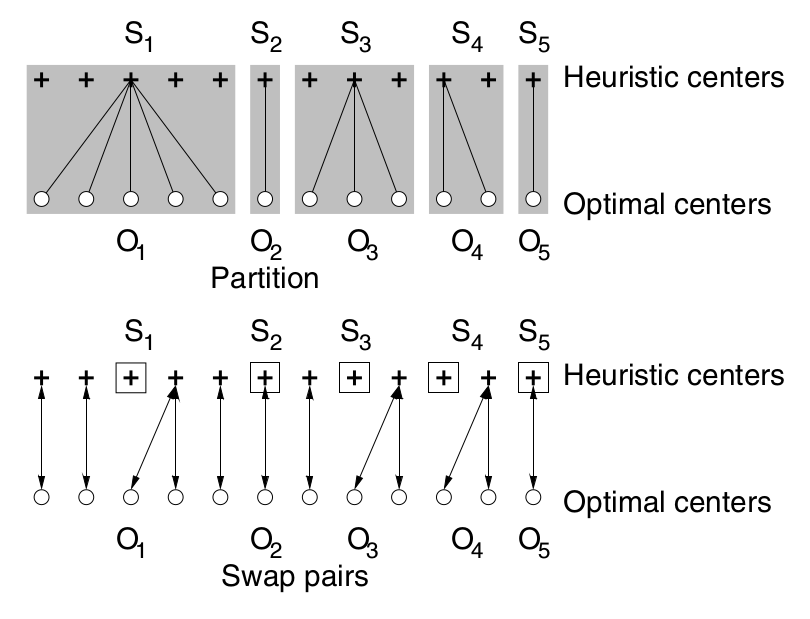
\includegraphics[totalheight=8cm]{swap.png}
        \caption{}
    \end{figure}
    Wyznaczymy teraz ograniczenie górne na zmianę funkcji $\Delta$ po wymianie punktów ze swap pary $(s, o)$.
    Zaczniemy od obliczenia najbliższych centrów z $S - \{s\} \cup \{o\}$ dla zadanego na wejściu zbioru $P$.
    Niech $N_{X}(x)$ będzie \textit{sąsiedztwem} punktu $x$, czyli podzbiorem punktów z $P$, dla których $x$ jest najbliższym punktem spośród punktów z $X$. 
    Dla punktów, które należą do $N_{C_{opt}}(o)$ zmiana $\Delta$ będzie następująca:
    \begin{equation}
        \sum_{q \in N_{C_{opt}}(o)} (\Delta(q, o) - \Delta(q, s_{q}))
    \end{equation}
    Każde $q \in N_{S}(s) \setminus N_{C_{opt}}(o)$ straciło przypisane mu centrum $s$ zatem punkt $q$ musi otrzymać nowe centrum.
    Niech $o_{q}$ będzie oznaczało najbliższe centrum dla punktu $q$.
    Skoro $q \notin N_{C_{opt}}(o)$ to $o_{q} \neq o$, zatem $s$ nie schwytało $o_{q}$.
    Zatem po skorzystaniu ze swap pary $(s,o)$, $s_{o_{q}}$, najbliższe heurystyczne centrum dla $o_{q}$ nadal istnieje.
    Zmiana $\Delta$ po wyborze nowych centrów jest co najwyżej równa:
    \begin{equation}
        \sum_{q \in N_{S}(s_{i}) \setminus N_{C_{opt}}(o_{i})} (\Delta(q, s_{o_{q}}) - \Delta(q, s))
    \end{equation}
    Na tym etapie dowodu koniecznie będzie wprowadzenie dwóch lematów.
    
    \begin{lemma}{\cite{Arya2004LocalSH}}
        Niech $S$ będzie zbiorem $k$ punktów spełniającym definicję 1-stable oraz niech $C_{opt}$ będzie optymalnym zbiorem dla problemu $k$-means.        Wtedy zachodzi następującą nierówność:
        \begin{equation}
            0 \leq \Delta(C_{opt}) - 3\Delta(S) + 2R
        \end{equation}
        gdzie $R = \sum_{q \in P} \Delta(q, s_{o_{q}})$.
    \end{lemma}
    \begin{proof}
        Na potrzeby dowodu ustalmy swap parę $(s, o)$.
        Ponieważ $S$ jest 1-stable to:
        \begin{equation}
           0 \leq \Delta(S) -  \Delta(S - \{s\} \cup \{o\})
        \end{equation}
        \begin{equation}
            = \sum_{q \in N_{C_{opt}}(o)} (\Delta(q, o) - \Delta(q, s_{q})) + \sum_{q \in N_{S}(s) \setminus N_{C_{opt}}(o)} (\Delta(q, s_{o_{q}}) - \Delta(q, s))
        \end{equation}
        Aby rozszerzyć sumę na wszystkie możliwe swap pary zauważmy, że dla każdego optymalnego centrum, jest ono wymienione tylko raz.
        Zatem każdy punkt $q$ kontrybuuje w pierwszej sumie tylko raz.
        Po drugie zaważmy, że różnca w drugiej sumie jest zawsze niezerowa dlatego rozszerzając zakres sumowania mozemy tylko zwiększyć sumaryczny wynik.
        \begin{equation}
            0 \leq \sum_{q \in P} (\Delta(q, o_{q}) - \Delta(q, s_{q})) + \sum_{q \in P} (\Delta(q, s_{o_{q}}) - \Delta(q, s_{q}))
        \end{equation}
        \begin{equation}
            0 \leq \sum_{q \in P} \Delta(q, o_{q}) - 3 \sum_{q \in P} \Delta(q, s_{q}) + 2\sum_{q \in P} \Delta(q, s_{o_{q}})
        \end{equation}
        \begin{equation}
            0 \leq \Delta(C_{opt}) - 3 \Delta(S) + 2R
        \end{equation}
    \end{proof}
    \noindent
    Wcześniej zdefiniowane $R$ nazywamy sumarycznym kosztem przepisania centrów.
    Korzystając z lematu 4.1 przekształcamy:
    \begin{equation}
        R = \sum_{o \in C_{opt}} \sum_{q \in N_{C_{opt}}(o)} \Delta(q, s_{o}) = \sum_{o \in O} \Delta(N_{C_{opt}}(o), s_{o}) 
    \end{equation}
    \begin{equation}
        = \sum_{o \in C_{opt}} (\Delta(N_{C_{opt}}(o), o) + |N_{o}(C_{opt})| \Delta(o, s_{o})
    \end{equation}
    \begin{equation}
        = \sum_{o \in C_{opt}} \sum_{q \in N_{C_{opt}}(o)} (\Delta(q, o) + \Delta(o, s_{o}))
    \end{equation}
    \begin{equation}
        \leq \sum_{o \in C_{opt}} \sum_{q \in N_{C_{opt}}(o)} (\Delta(q, o) + \Delta(o, s_{q}))
    \end{equation}
    \begin{equation}
        = \sum_{q \in P} (\Delta(q, o_{q}) + \Delta(o_{q}, s_{q}))
    \end{equation}
    gdzie ostatnia nierówność bazuje na fakcie, że dla każdego $q \in N_{C_{opt}}(o)$ mamy $\Delta(o, s_{o}) \leq \Delta(o, s_{q})$.
    Następnie korzystamy z nierówności trójkąta.
    \begin{equation}
        R \leq  \sum_{q \in P} \Delta(q, o_{q}) + \sum_{q \in P} ( d(o_{q}, q) + d(q, s_{q}))^{2}
    \end{equation}
    \begin{equation}
        = \sum_{q \in P} \Delta(q, o_{q}) + \sum_{q \in P} ( d(o_{q}, q)^{2} + 2d(o_{q}, q)d(q, s_{q}) + d(q, s_{q})^{2})
    \end{equation}
    \begin{equation}
        = 2\sum_{q \in P} \Delta(q, o_{q}) + \sum_{q \in P} \Delta(q, s_{q}) + 2\sum_{q \in P} d(o_{q}, q)d(q, s_{q})
    \end{equation}
    \begin{equation}
        = 2\Delta(C_{opt}) + \Delta(S) + 2\sum_{q \in P} d(o_{q}, q)d(q, s_{q})
    \end{equation}
    \begin{lemma}{\cite{Arya2004LocalSH}}
        Niech $\langle o_{i} \rangle$ oraz $\langle s_{i} \rangle$ będą ciągami liczb rzeczywistych, dla których zachodzi:
        \begin{equation}
            \delta^2 = \frac{\sum_{i} s_{i}^{2}}{\sum_{i} o_{i}^{2}}
        \end{equation}
        dla pewnego $\delta > 0$.
        Wtedy:
        \begin{equation}
            \sum_{i=1}^{n} o_{i} s_{i} \leq \frac{1}{\delta} \sum_{i=1}^{n} s_{i}^{2}
        \end{equation}
    \end{lemma}
    \begin{proof}
        Z nierówności Schwarza:
        \begin{equation}
            \sum_{i=1}^{n} o_{i} s_{i} \leq \Big( \sum_{i=1}^{n} o_{i}^{2} \Big)^{\frac{1}{2}} \Big( \sum_{i=1}^{n} s_{i}^{2} \Big)^{\frac{1}{2}}
        \end{equation}
        \begin{equation}
            = \Big( \frac{1}{\delta^{2}}\sum_{i=1}^{n} s_{i}^{2} \Big)^{\frac{1}{2}} \Big( \sum_{i=1}^{n} s_{i}^{2} \Big)^{\frac{1}{2}}
        \end{equation}
        \begin{equation}
            = \frac{1}{\delta} \sum_{i=1}^{n} s_{i}^{2}
        \end{equation}
    \end{proof}
    Niech $\langle o_{i} \rangle$ będzie ciągiem $d(q, o_{q})$ oraz niech $\langle s_{i} \rangle$ będzie ciągiem $d(q,s_{q})$ dla wszystkich $q \in P$.
    Z tego wynika, że współczynnik aproksymacji możemy przedstawić jako:
    \begin{equation}
        \alpha = \delta^{2} = \frac{\Delta(S)}{\Delta(C_{opt})} = \frac{\sum_{q \in P} d(q,s_{q})^{2}}{\sum_{q \in P} d(q,o_{q})^{2}} =\frac{\sum_{i=1}^{n} s_{i}^{2}}{\sum_{i=1}^{n} o_{i}^{2}}
    \end{equation}
    gdzie $S$ jest zbiorem 1-stable uzyskanym przez wcześniej przedstawiony algorytm.
    Korzystając z lematu 4.3:
    \begin{equation}
        R \leq 2\Delta(C_{opt}) + \Delta(S) + 2\sum_{q \in P} d(o_{q}, q)d(q, s_{q}) 
    \end{equation}
    \begin{equation}
        \leq 2\Delta(C_{opt}) + \Delta(S) + \frac{2}{\delta}\sum_{q \in P} d(q, s_{q})^{2} 
    \end{equation}
    \begin{equation}
        = 2\Delta(C_{opt}) + \Delta(S) + \frac{2}{\delta}\Delta(S)
    \end{equation}
    \begin{equation}
        = 2\Delta(C_{opt}) + \Big(1 + \frac{2}{\delta} \Big)\Delta(S)
    \end{equation}
    Z lematu 4.2 wiemy, że:
    \begin{equation}
        0 \leq \Delta(C_{opt}) - 3\Delta(S) + 2R
    \end{equation}
    \begin{equation}
        = \Delta(C_{opt}) - 3\Delta(S) + 2\Big(2\Delta(C_{opt}) + \Big(1 + \frac{2}{\delta} \Big)\Delta(S)\Big)
    \end{equation}
    \begin{equation}
        \leq 5\Delta(C_{opt}) - \Big(1 - \frac{4}{\delta} \Big)\Delta(S)
    \end{equation}
    Powyższą nierówności możemy przekształcić do postaci:
    \begin{equation}
        \frac{5}{1-\frac{4}{\delta}} \geq \frac{\Delta(S)}{\Delta(C_{opt})} = \delta^{2}
    \end{equation}
    \begin{equation}
        5 \geq \delta^{2} \Big(1 - \frac{4}{\delta} \Big)
    \end{equation}
    \begin{equation}
        0 \geq (\delta - 5)(\delta + 1)
    \end{equation}
    To implikuje, że $\delta \leq 5$, zatem współczynnik omawianego algorytmu możemy ograniczyć przez $\alpha = \delta^{2} \leq 25$, co kończy dowód twierdzenia 4.2.
\end{proof}